%!\subsection{Future Trends and speculations}
%!\label{subsec:Futuretrends}

%!==========================
%Speculate on the potential future trajectories of architectural design, digital fabrication, and mixed reality. Discuss how these trends might shape the built environment, and propose ideas for further research and exploration.
%!==========================

%!\subsection{Object-Oriented Ontology}
%!\label{subsec:ObjectOrientedOntology}
% add the concept of Object-Oriented. Using these concepts as basis. I want to express that the mr experiment is based on the idea that architecture as a tool should be invisible and confortable while in use. But it should  create emotion when seen as part of the landscape as a form of art to recapture the humand oriented city .

It may be cheaper and quicker to build a load-bearing brick wall, but
the High Tech architect will always prefer the steel frame and the lightweight metal panel because this is a technique more in tune with the spirit of the age.
He is committed to the idea that building must eventually catch up with the rest of technology, and he is determined to "drag building into the twentieth century".\cite{Davies1988}

Heideggers tool analysis states that as the tool is a tool it disappears in favor of some purpose he continues to explain that generally we don't notice equipment until it fails, like when An earthquake calls attention to the ground we walk or when a medical problem alerts us of the presence of organs that we have silently depended\cite{Harman2011}.
Harmans, Object-oriented ontology, borrows this concept to formulate its central claim that objects have hidden qualities and realities, and they withdraw from our understanding.\cite{Gage2015}
he idea that we live our lives on a layer of invisible equipment has significant ramifications for architecture, a discipline that produces the equipment on and in which we exist.\cite{Gage2015}

(Figure \ref{fig:complexornament})

%% Figure of Contemporary timeline
     \begin{figure*}[htb]
          \centering
          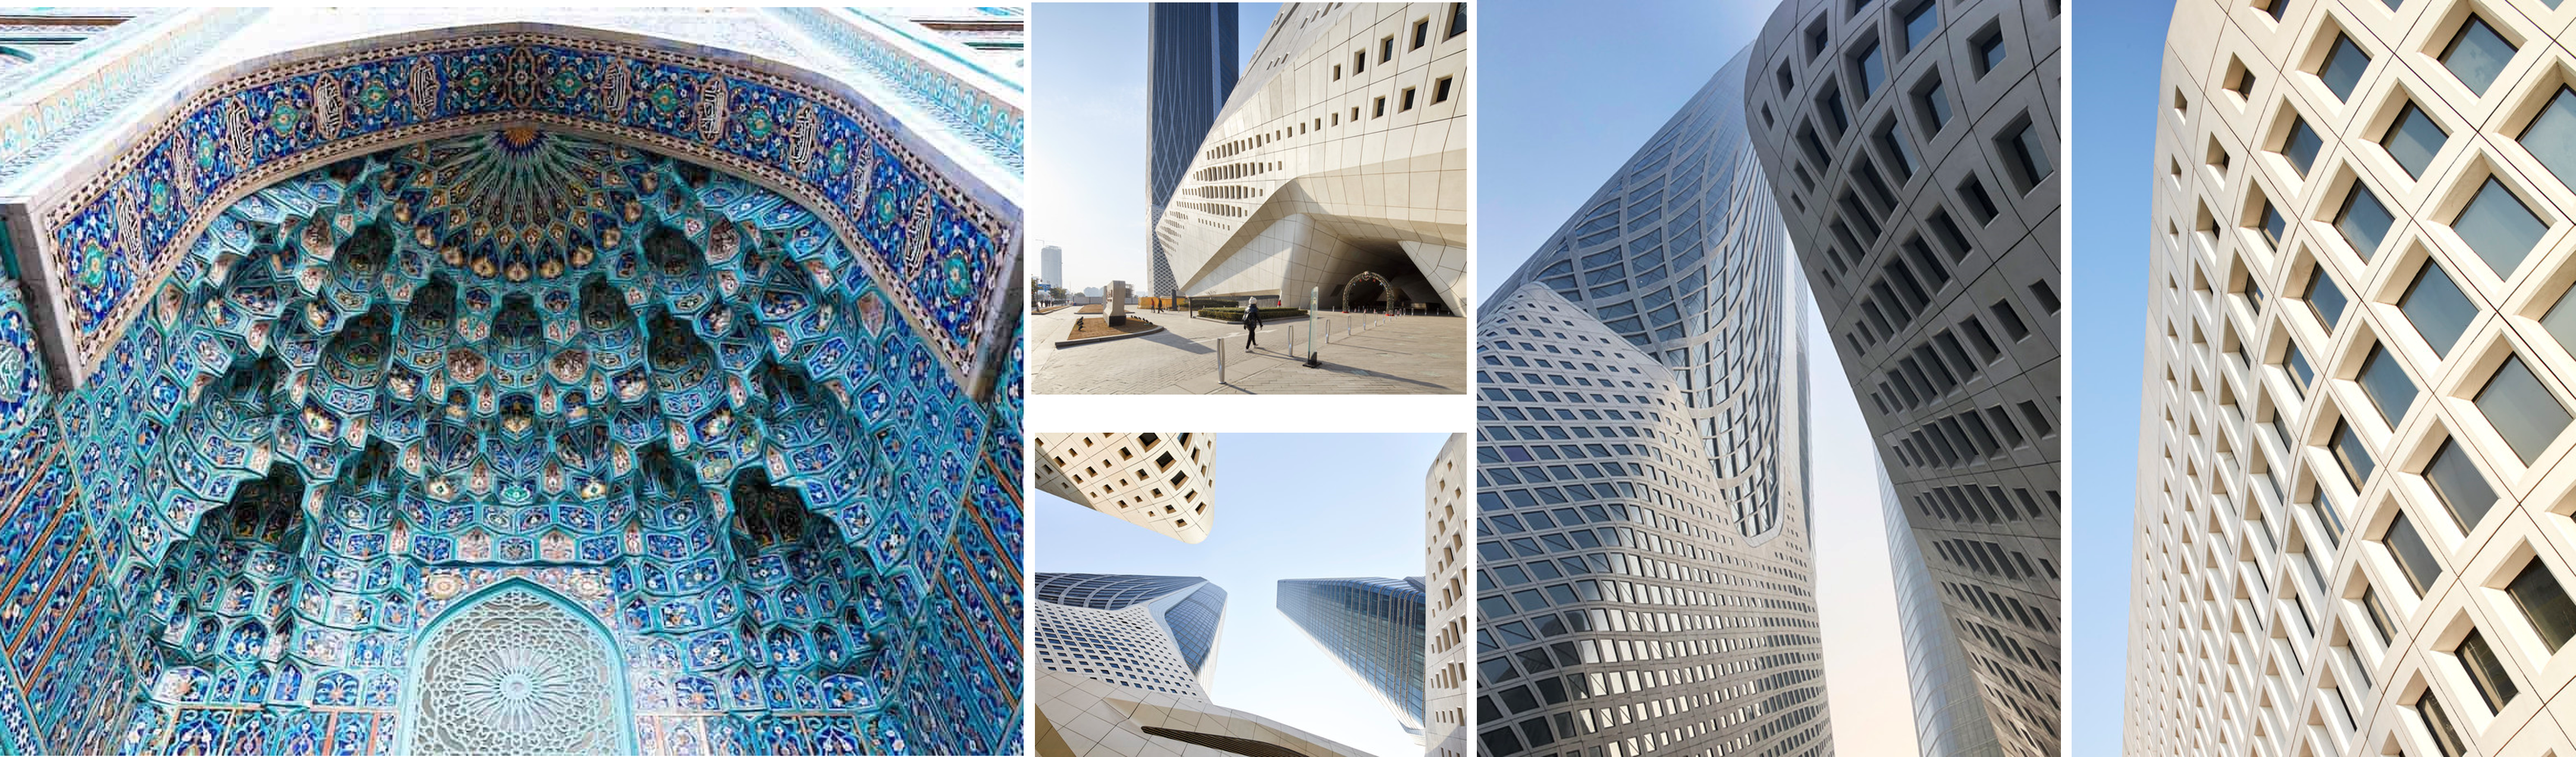
\includegraphics[width= \linewidth]{Images/complexornament}
          \caption{Complex ornament reference  (\textit{Images edited from source)}}
          \label{fig:complexornament}
        \end{figure*}
